\documentclass[journal, a4paper]{IEEEtran}

% some very useful LaTeX packages include:

%\usepackage{cite}      % Written by Donald Arseneau
                        % V1.6 and later of IEEEtran pre-defines the format
                        % of the cite.sty package \cite{} output to follow
                        % that of IEEE. Loading the cite package will
                        % result in citation numbers being automatically
                        % sorted and properly "ranged". i.e.,
                        % [1], [9], [2], [7], [5], [6]
                        % (without using cite.sty)
                        % will become:
                        % [1], [2], [5]--[7], [9] (using cite.sty)
                        % cite.sty's \cite will automatically add leading
                        % space, if needed. Use cite.sty's noadjust option
                        % (cite.sty V3.8 and later) if you want to turn this
                        % off. cite.sty is already installed on most LaTeX
                        % systems. The latest version can be obtained at:
                        % http://www.ctan.org/tex-archive/macros/latex/contrib/supported/cite/

\usepackage{graphicx}   % Written by David Carlisle and Sebastian Rahtz
                        % Required if you want graphics, photos, etc.
                        % graphicx.sty is already installed on most LaTeX
                        % systems. The latest version and documentation can
                        % be obtained at:
                        % http://www.ctan.org/tex-archive/macros/latex/required/graphics/
                        % Another good source of documentation is "Using
                        % Imported Graphics in LaTeX2e" by Keith Reckdahl
                        % which can be found as esplatex.ps and epslatex.pdf
                        % at: http://www.ctan.org/tex-archive/info/

%\usepackage{psfrag}    % Written by Craig Barratt, Michael C. Grant,
                        % and David Carlisle
                        % This package allows you to substitute LaTeX
                        % commands for text in imported EPS graphic files.
                        % In this way, LaTeX symbols can be placed into
                        % graphics that have been generated by other
                        % applications. You must use latex->dvips->ps2pdf
                        % workflow (not direct pdf output from pdflatex) if
                        % you wish to use this capability because it works
                        % via some PostScript tricks. Alternatively, the
                        % graphics could be processed as separate files via
                        % psfrag and dvips, then converted to PDF for
                        % inclusion in the main file which uses pdflatex.
                        % Docs are in "The PSfrag System" by Michael C. Grant
                        % and David Carlisle. There is also some information
                        % about using psfrag in "Using Imported Graphics in
                        % LaTeX2e" by Keith Reckdahl which documents the
                        % graphicx package (see above). The psfrag package
                        % and documentation can be obtained at:
                        % http://www.ctan.org/tex-archive/macros/latex/contrib/supported/psfrag/

%\usepackage{subfigure} % Written by Steven Douglas Cochran
                        % This package makes it easy to put subfigures
                        % in your figures. i.e., "figure 1a and 1b"
                        % Docs are in "Using Imported Graphics in LaTeX2e"
                        % by Keith Reckdahl which also documents the graphicx
                        % package (see above). subfigure.sty is already
                        % installed on most LaTeX systems. The latest version
                        % and documentation can be obtained at:
                        % http://www.ctan.org/tex-archive/macros/latex/contrib/supported/subfigure/

\usepackage{url}        % Written by Donald Arseneau
                        % Provides better support for handling and breaking
                        % URLs. url.sty is already installed on most LaTeX
                        % systems. The latest version can be obtained at:
                        % http://www.ctan.org/tex-archive/macros/latex/contrib/other/misc/
                        % Read the url.sty source comments for usage information.

%\usepackage{stfloats}  % Written by Sigitas Tolusis
                        % Gives LaTeX2e the ability to do double column
                        % floats at the bottom of the page as well as the top.
                        % (e.g., "\begin{figure*}[!b]" is not normally
                        % possible in LaTeX2e). This is an invasive package
                        % which rewrites many portions of the LaTeX2e output
                        % routines. It may not work with other packages that
                        % modify the LaTeX2e output routine and/or with other
                        % versions of LaTeX. The latest version and
                        % documentation can be obtained at:
                        % http://www.ctan.org/tex-archive/macros/latex/contrib/supported/sttools/
                        % Documentation is contained in the stfloats.sty
                        % comments as well as in the presfull.pdf file.
                        % Do not use the stfloats baselinefloat ability as
                        % IEEE does not allow \baselineskip to stretch.
                        % Authors submitting work to the IEEE should note
                        % that IEEE rarely uses double column equations and
                        % that authors should try to avoid such use.
                        % Do not be tempted to use the cuted.sty or
                        % midfloat.sty package (by the same author) as IEEE
                        % does not format its papers in such ways.

\usepackage{amsmath}    % From the American Mathematical Society
                        % A popular package that provides many helpful commands
                        % for dealing with mathematics. Note that the AMSmath
                        % package sets \interdisplaylinepenalty to 10000 thus
                        % preventing page breaks from occurring within multiline
                        % equations. Use:
%\interdisplaylinepenalty=2500
                        % after loading amsmath to restore such page breaks
                        % as IEEEtran.cls normally does. amsmath.sty is already
                        % installed on most LaTeX systems. The latest version
                        % and documentation can be obtained at:
                        % http://www.ctan.org/tex-archive/macros/latex/required/amslatex/math/


\makeatletter
\newif\if@restonecol
\makeatother
\let\algorithm\relax
\let\endalgorithm\relax
\usepackage[linesnumbered,ruled,vlined]{algorithm2e}%[ruled,vlined]{
\usepackage{algpseudocode}
\usepackage{amsmath}
\renewcommand{\algorithmicrequire}{\textbf{Input:}}  % Use Input in the format of Algorithm
\renewcommand{\algorithmicensure}{\textbf{Output:}} % Use Output in the format of Algorithm 
% Other popular packages for formatting tables and equations include:

%\usepackage{array}
% Frank Mittelbach's and David Carlisle's array.sty which improves the
% LaTeX2e array and tabular environments to provide better appearances and
% additional user controls. array.sty is already installed on most systems.
% The latest version and documentation can be obtained at:
% http://www.ctan.org/tex-archive/macros/latex/required/tools/

% V1.6 of IEEEtran contains the IEEEeqnarray family of commands that can
% be used to generate multiline equations as well as matrices, tables, etc.

% Also of notable interest:
% Scott Pakin's eqparbox package for creating (automatically sized) equal
% width boxes. Available:
% http://www.ctan.org/tex-archive/macros/latex/contrib/supported/eqparbox/

% *** Do not adjust lengths that control margins, column widths, etc. ***
% *** Do not use packages that alter fonts (such as pslatex).         ***
% There should be no need to do such things with IEEEtran.cls V1.6 and later.


% Your document starts here!
\begin{document}
\begin{titlepage}

\newcommand{\HRule}{\rule{\linewidth}{0.5mm}} % Defines a new command for the horizontal lines, change thickness here

\center % Center everything on the page
 %----------------------------------------------------------------------------------------
%	LOGO SECTION
%----------------------------------------------------------------------------------------

~\\[1cm]

\includegraphics{SCUT.png}\\[2cm] % Include a department/university logo - this will require the graphicx package

%----------------------------------------------------------------------------------------
%	TITLE SECTION
%----------------------------------------------------------------------------------------

\HRule \\[1cm]
{ \huge \bfseries The Experiment Report of \textit{Machine Learning} }\\[0.6cm] % Title of your document
\HRule \\[2cm]
%----------------------------------------------------------------------------------------
%	HEADING SECTIONS
%----------------------------------------------------------------------------------------


\textsc{\LARGE \textbf{School:} School of Software Engineering}\\[1cm]
\textsc{\LARGE \textbf{Subject:} Software Engineering}\\[2cm] 

 
%----------------------------------------------------------------------------------------
%	AUTHOR SECTION
%----------------------------------------------------------------------------------------

\begin{minipage}{0.4\textwidth}
\begin{flushleft} \large
\emph{Author:}\\
Lizhao Liu % Your name
\end{flushleft}
\end{minipage}
~
\begin{minipage}{0.4\textwidth}
\begin{flushright} \large
\emph{Supervisor:} \\
Mingkui Tan % Supervisor's Name
\end{flushright}
\end{minipage}\\[2cm]
~
\begin{minipage}{0.4\textwidth}
\begin{flushleft} \large
\emph{Student ID:}\\
201730683109
\end{flushleft}
\end{minipage}
~
\begin{minipage}{0.4\textwidth}
\begin{flushright} \large
\emph{Grade:} \\
Undergraduate
\end{flushright}
\end{minipage}\\[2cm]

% If you don't want a supervisor, uncomment the two lines below and remove the section above
%\Large \emph{Author:}\\
%John \textsc{Smith}\\[3cm] % Your name

%----------------------------------------------------------------------------------------
%	DATE SECTION
%----------------------------------------------------------------------------------------

{\large \today}\\[2cm] % Date, change the \today to a set date if you want to be precise

 
%----------------------------------------------------------------------------------------

\vfill % Fill the rest of the page with whitespace

\end{titlepage}

% Define document title and author
	\title{Logistic Regression and SVM}
	\maketitle

% Write abstract here
\begin{abstract}
In this report, we solve the binary classification problem in a9a dataset by Logistic Regression (LR) and Support Vector Machine (SVM). \\
We perform experiments on three aspects: \\
1. Loss function comparision in SVM. \\
2. Hyper-parameter tuning in SVM. \\
3. Initilizer comparision in both LR and SVM. \\
4. Optimizer comparision in both LR and SVM. \\
\end{abstract}

% Each section begins with a \section{title} command
\section{Introduction}
	% \PARstart{}{} creates a tall first letter for this first paragraph
\PARstart{L}{inear} Regression is the core of machine learning. Based on it, many machine learning algorithms, such as RR, Logistics Regression, SVM are developed. Even in many deep learning models, such as Covolutional Neural Network (CNN), Long Short Term Memory (LSTM), Gated Recurrent Unit (GRU), LR (or Linear Layer) is the basic component. So it is very important to fully exploit the insight of LR. To achieve that goal, In this experiment, we conduct many experiments on CSF optimized LR, CSF optimized RR, MBGD optimized LR by solving the house price predicting problem.

% Main Part
\section{Methods and Theory}
In this part, we first define the LR, Mean Squared Error (MES) loss function. Then we solve the closed form solution for LR and its variant RR. At last we define GD algorithm, and its variants SGD and MBGD.
\subsection{Linear Regression}
Given dataset $ D=\{x_{i}, y_{i}\}_{i=1}^{m}$, where $x_{i} \in \mathbf{R}^{n}$ and $y_{i} \in \mathbf{R}$.
Liner Regression Model is parameterized by $(W, b)$, where $W \in \mathbf{R}^{n}$ and $b \in \mathbf{R}$ and the form of it is:
 \begin{center}
 	\begin{equation}
 	y_{i} = x_{i}^{T}W + b
 	\end{equation}
 \end{center} 
We can write it in vertorized form:
 \begin{center}
	\begin{equation}
	y = X^{T}W
	\end{equation}
\end{center} 
where \\
$\mathbf {y} ={\begin{pmatrix}y_{1}\\y_{2}\\\vdots \\y_{m}\end{pmatrix}},\quad 
{\displaystyle {\boldsymbol {W }}={\begin{pmatrix}b \\W_{1}\\W_{2}\\\vdots \\W_{n}\end{pmatrix}},} \\
{\displaystyle X={\begin{pmatrix}1&\mathbf{x} _{1}^{\mathsf {T}}\\1&\mathbf {x} _{2}^{\mathsf {T}}\\\vdots&\vdots \\1&\mathbf {x} _{m}^{\mathsf {T}}\end{pmatrix}}={\begin{pmatrix}1&x_{11}&\cdots &x_{1n}\\1&x_{21}&\cdots &x_{2n}\\\vdots &\vdots &\ddots &\vdots \\1&x_{m1}&\cdots &x_{mn}\end{pmatrix}}.} \\
$
\subsection{Mean Squared Error}
Given the prediction of Linear Model $\hat{y} = X^{T}W $ and the Ground truth $y$, the MSE loss function is:
 \begin{center}
	\begin{equation}
	L(\hat{y}, y) = \frac{1}{2m} \Sigma_{i=1}^{m}(\hat{y}_i, y_i) 
				= \frac{1}{2m}(\hat{y} - y)^{T}(\hat{y} - y)
	\end{equation}
\end{center} 
\subsection{Closed form Solution}
The best parameter $W^{*}$ can be obtained by \\
\begin{equation}
 W^{*} = \arg\min_{W}L(X^{T}W, y)  
\end{equation} \par
So, we set 
\begin{equation}
\frac{\partial L(\hat{y}, y)}{\partial W} = 0 \\
\end{equation} \par
We can get 
\begin{equation}
\label{eq:cfs}
W^{*} = (X^{T}X)^{-1}X^{T}y
\end{equation}
\subsection{Ridge Regression}
In Equation~\ref{eq:cfs}, when $n > m$, $X^{T}X$ is not invertible. Ridge Regression tackle this problem by adding a small term. So the CFS for RR is
\begin{equation}
W_{ridge}^{*} = (X^{T}X + \lambda \mathbf{I})^{-1}X^{T}y
\end{equation} \par
Where $\mathbf{I}$ is identity matrix. \par
In this way, the loss function for Ridge Regression is
\begin{equation}
L_{ridge}(\hat{y}, y) = \frac{1}{2m}(\hat{y} - y)^{T}(\hat{y} - y)  + \frac{1}{2} W^{T} W
\end{equation} \par
In another point of view, RR can be seen as a regularized version of LR.
\subsection{Gradient Descent}
Not all problem can be derived a CFS, which is often the case in machine learning. So instead of getting the best parameters $W^{*}$ immedeatly, we can update it incremently until $W$ gets close enough to $W^{*}$. That is the basic idea of GD algorithm. GD algorithm can be found in Algorithm~\ref{alg: Gradient_Descent}. 
\begin{algorithm}

	\label{alg: Gradient_Descent}
	\caption{Gradient Descent}
	\KwIn{Training Dataset $ D=\{x_{i}, y_{i}\}_{i=1}^{m}$, learning rate $\eta $, max iteration $ N$, parameter $W$}
	\KwOut{Optimized parameter $\hat{W}$}
	$t \gets 1$ \\
	\For{$t < N $}
	{
		$\hat{y} \gets X^{T}W $ \\
		$ L(\hat{y}, y) \gets \frac{1}{2m}(\hat{y} - y)^{T}(\hat{y} - y)$ \\
		$\Delta{W} \gets \frac{\partial L}{\partial W}$ \\
		$W \gets W - \eta * \Delta{W}$ \\
	}
	$\hat{W} \gets W$ \\
	return $\hat{W}$
\end{algorithm}

\subsection{Stochastic Gradient Descent}
Different from GD which updates after it computes the gradient of parameters over all examples, stochastic gradient descent updates immediately once it computes parameters' gradient from only one example. SGD algorithm can be found in Algorithm~\ref{alg: Stochastic_Gradient_Descent}. It can be seen in the algorithm that, there is another for loop inside the for loop of GD algorithm, which leads to time un-efficiency.
\begin{algorithm}
		\label{alg: Stochastic_Gradient_Descent}
	\caption{Stochastic Gradient Descent}
	\KwIn{Training Dataset $ D=\{x_{i}, y_{i}\}_{i=1}^{m}$, learning rate $\eta $, max iteration $ N$, parameter $W$}
	\KwOut{Optimized parameter $\hat{W}$}
	$t \gets 1$ \\
	\For{$t < N $}
	{
		$ i \gets 0 $ \\
		\For{$ i < m $}
		{
			$\hat{y}_{i} \gets X^{T}_{i}W $ \\
			$ L(\hat{y}_{i}, y_{i}) \gets \frac{1}{2}(\hat{y}_{i} - y_{i})^{T}(\hat{y}_{i} - y_{i})$ \\
			$\Delta{W} \gets \frac{\partial L}{\partial W}$ \\
			$W \gets W - \eta * \Delta{W}$ \\
		}
	}
	$\hat{W} \gets W$ \\
	return $\hat{W}$
\end{algorithm}

\subsection{Mini Batch Gradient Descent}
Due to the fact that SGD updates the parameters based on only one examples, which it is time-comsuming, mini batch gradient descent updates the parameter based on a batch of examples, typically the batch size is bigger than 1 and smaller than the number of whole examples, e.g. 8, 16, 32... MBGD Algorithm can be found in Algorithm~\ref{alg: Mini_Batch_Gradient_Descent}.
\begin{algorithm}
	\label{alg: Mini_Batch_Gradient_Descent}
	\caption{Mini Batch Gradient Descent}
	\KwIn{Training Dataset $ D=\{x_{i}, y_{i}\}_{i=1}^{m}$, learning rate $\eta $, max iteration $ N$, parameter $W$}
	\KwOut{Optimized parameter $\hat{W}$}
	$t \gets 1$ \\
	\For{$t < N $}
	{
		$ i \gets 0 $ \\
		\For{$ X_{batch}, y_{batch} $ in $D$}
		{
			$\hat{y}_{batch} \gets X^{T}_{batch}W $ \\
			$ L(\hat{y}_{batch}, y_{batch}) \gets \frac{1}{2}(\hat{y}_{batch} - y_{batch})^{T}(\hat{y}_{batch} - y_{batch})$ \\
			$\Delta{W} \gets \frac{\partial L}{\partial W}$ \\
			$W \gets W - \eta * \Delta{W}$ \\
		}
	}
	$\hat{W} \gets W$ \\
	return $\hat{W}$
\end{algorithm}


\section{Experiments}
\subsection{Dataset}
We conduct all the experiments on housing dataset, which has total 506 examples and each example's form is $(x, y)$, where $x \in \mathbf{R}^{13}$ and $y \in \mathbf{R}$. We split the dataset into three part: 272 training examples, 67 validation examples and 167 test examples. $X$ is already scaled between $-1$ and $1$. And we normalized the $X_{train}, X_{val}, X_{test} $ by using the mean and variance of $X_{train}$. 

\subsection{Implementation}
We implement the LR, RR and GD, GD, MBGD algorithm using python and mainly rely on the numpy package.

\subsection{Linear Regression and Ridge Regression}
In this section, we conduct the experiment of serveral magnitude of $\lambda$ of RR in training set, which leads to serveral $W_{ridge}$. We use $L_2{norm}$ to represent the magnitude of a vector. Given $v \in \mathbf{R}^{n}$
\begin{equation}
	L_2norm(v) = \sqrt{\Sigma_{i=1}^{n} v_{i}}
\end{equation} \par
From Table~\ref{tab:Ridge_Regression}, we can see that: \par
First, as the magnitude of lambda becomes bigger, both $MSE_{train}$ and $MSE_{val}$ become bigger. \par
Second, as the magnitude of lambda becomes bigger, the magnitude of $W_{ridge}$ become smaller. \par
The first observation is not often the cases. But the second observation can be explained that as the regularizer $\lambda$ become bigger, the $W$ is regularized, so that it is smaller. \par
By comparing Table~\ref{tab:Ridge_Regression} and Table~\ref{tab:Linear_Regression}, we can see that, the performance and the weight magnitude is almost the same as the $\lambda$ is small, but the difference become larger as $\lambda$ grows. \par
We also explore the weight mantitude between LR and RR under different $\lambda$ magnitude setting. Specifically, we set $log_{10}^{\lambda}$ in range from -7 to 3. We can see from Fig~\ref{fig:ridge_w}, as the magnitude of $\lambda$ growing, the weight magnitude of ridge regression become much smaller than linear regression. \par
\begin{table}[!hbt]
	% Center the table
	\begin{center}
		% Title of the table
		\caption{Different lambdas' impact in terms of error and $W$ magnitude. Best result are in bold.}
		\label{tab:Ridge_Regression}
		% Table itself: here we have two columns which are centered and have lines to the left, right and in the middle: |c|c|
		\begin{tabular}{|c|c|c|c|c|c|c|c|}
			% To create a horizontal line, type \hline
			\hline
			% To end a column type &
			% For a linebreak type \\
			$log_{10}^{\lambda}$ & -2 & -1 & 0 & 1 & 2 & 3 \\
			\hline
			$MSE_{train}$   & \textbf{10.23} & \textbf{10.23} & 10.24 & 10.63 & 30.37 & 181.35   \\
			\hline
			$MSE_{val}$  & \textbf{17.08} & 17.09 & 17.16 & 18.20 & 43.92 & 214.55   \\
			\hline
			$L_2norm(W_{ridge})$  & 0.83 & 0.82 & 0.81 & 0.72 & 0.50 & 0.38 \\
			\hline
		\end{tabular}
	\end{center}
\end{table}

\begin{table}[!hbt]
	% Center the table
	\begin{center}
		% Title of the table
		\caption{Linear Regression Error and $W$ magnitude.}
		\label{tab:Linear_Regression}
		% Table itself: here we have two columns which are centered and have lines to the left, right and in the middle: |c|c|
		\begin{tabular}{|c|c|}
			% To create a horizontal line, type \hline
			\hline
			$MSE_{train}$ & 10.23    \\
			\hline
			$MSE_{val}$ & 17.08    \\
			\hline
			$L_2norm(W)$ & 0.83  \\
			\hline
		\end{tabular}
	\end{center}
\end{table}

\begin{figure}[!hbt]
	% Center the figure.
	\begin{center}
		% Include the eps file, scale it such that it's width equals the column width. You can also put width=8cm for example...
		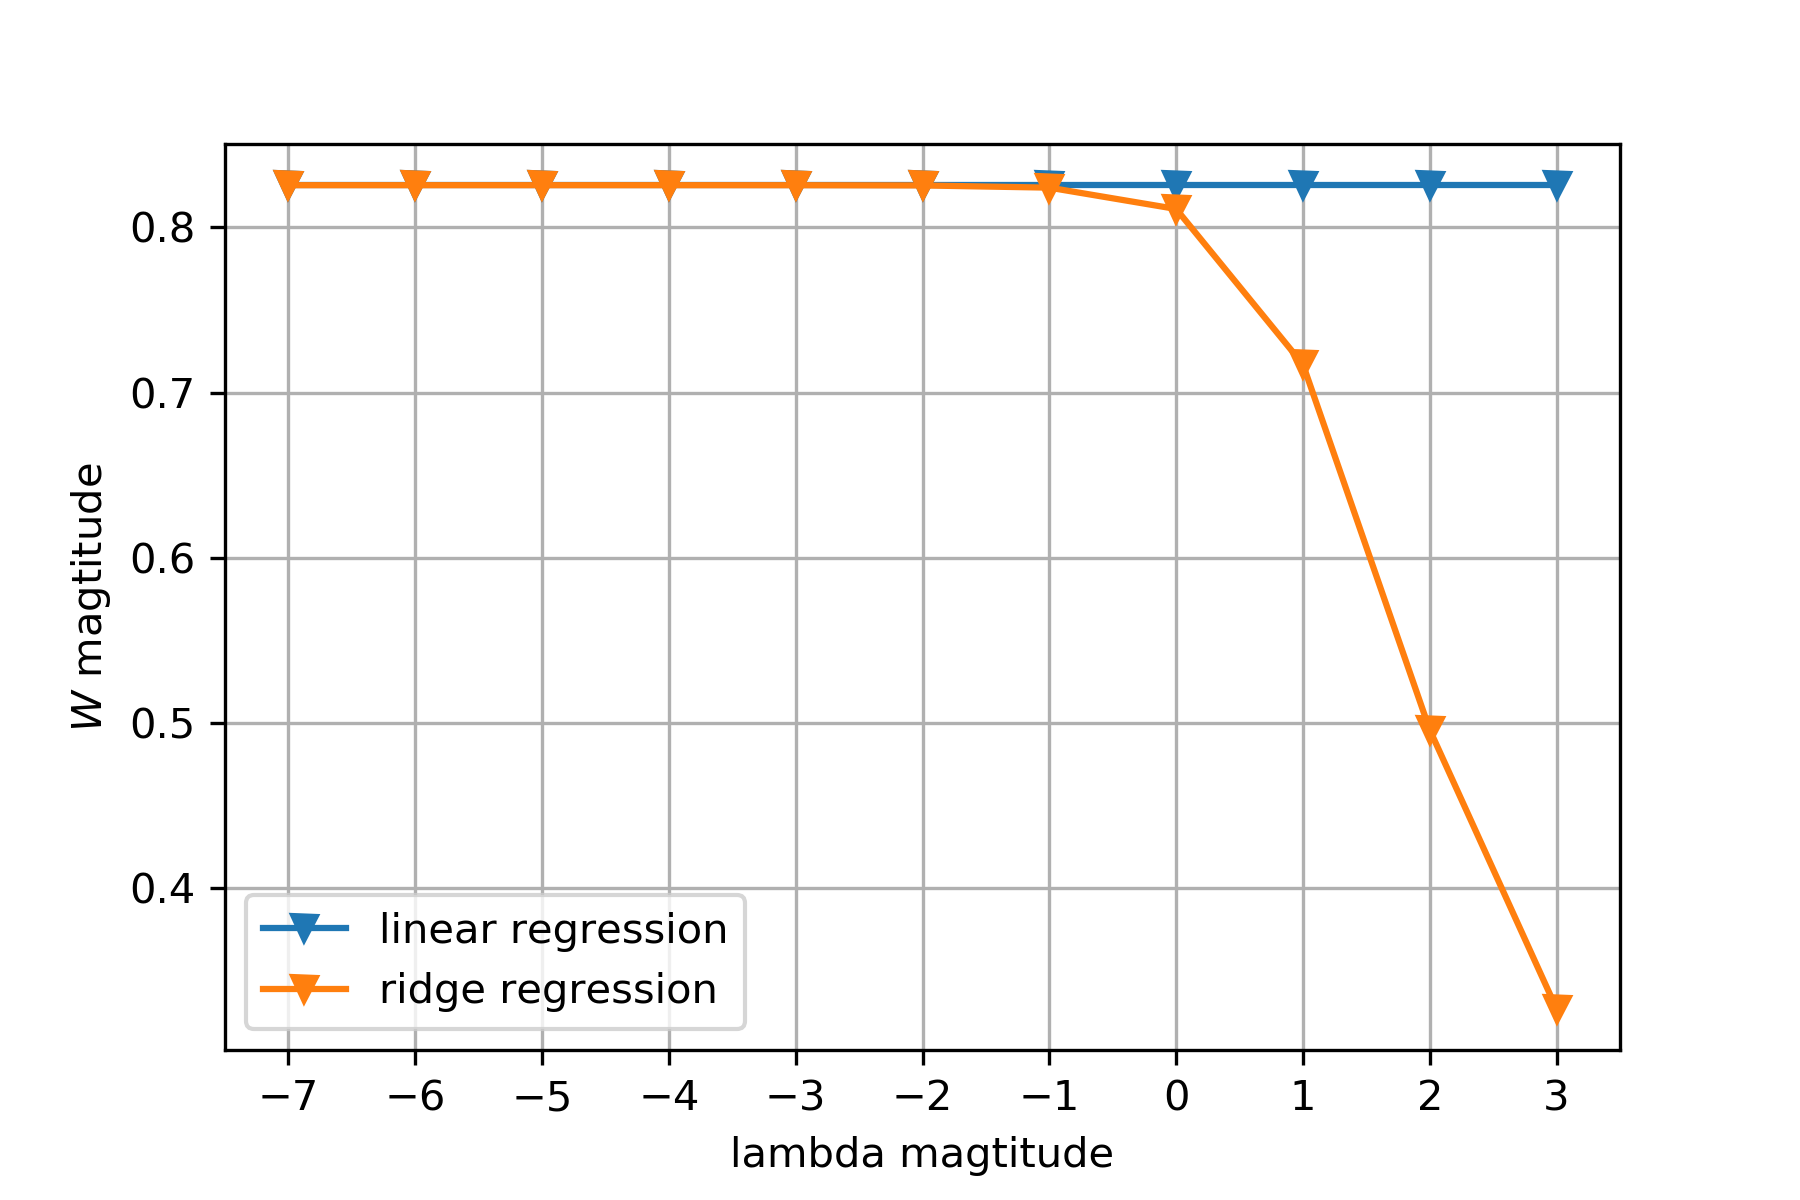
\includegraphics[width=\columnwidth]{ridge_w}
		% Create a subtitle for the figure.
		\caption{The magnitude of $W_{ridge}$ under different lambda mgnitude.}
		% Define the label of the figure. It's good to use 'fig:title', so you know that the label belongs to a figure.
		\label{fig:ridge_w}
	\end{center}
\end{figure} 

\subsection{Gradient Descent, Stochastic Gradient Descent and Mini Batch Gradient Descent}
In this section, we conduct experiments on optimizing the LR model by using GD, SGD, MBGD  algorrithms, and compare them in terms of convergence and time cost. \par
We first evaluate the convergence of three algorithms, specificlly we set batch size in a range from 1 to number of full examples in training set. When the batch size is one, mini batch gradient descent becomes stochastic gradient descent and when the batch size equals to number of full examples, mini batch gradient descent becomes gradient descent. All experiments are with the same learning rate 0.01.\par
As we can see from Fig~\ref{fig:batch_size_train} and Fig~\ref{fig:batch_size_val}, as the batch size become larger, the convergence of the linear regression model bocome slower. The reason is that, in each epoch, the smaller the batch size, the model have more update steps, so the convergence is faster. Especially, the stochastic gradient descent converges within 10 steps, while gradient descent requires nearly 400 steps, there is a 400x margin.\par
We then measure the time cost for each batch size. \par 
As illustrated in Fig~\ref{fig:time_cost}, the smaller the batch size, more time cost is required, because of the explicit for loop in the SGD and MBGD. Especially, the GD requires only about 1 seconds in one step, while SGD requires 60 seconds, there exist a 60x margin.  \par
% This is how you include a eps figure in your document. LaTeX only accepts EPS or TIFF files.
\begin{figure}[!hbt]
	% Center the figure.
	\begin{center}
		% Include the eps file, scale it such that it's width equals the column width. You can also put width=8cm for example...
		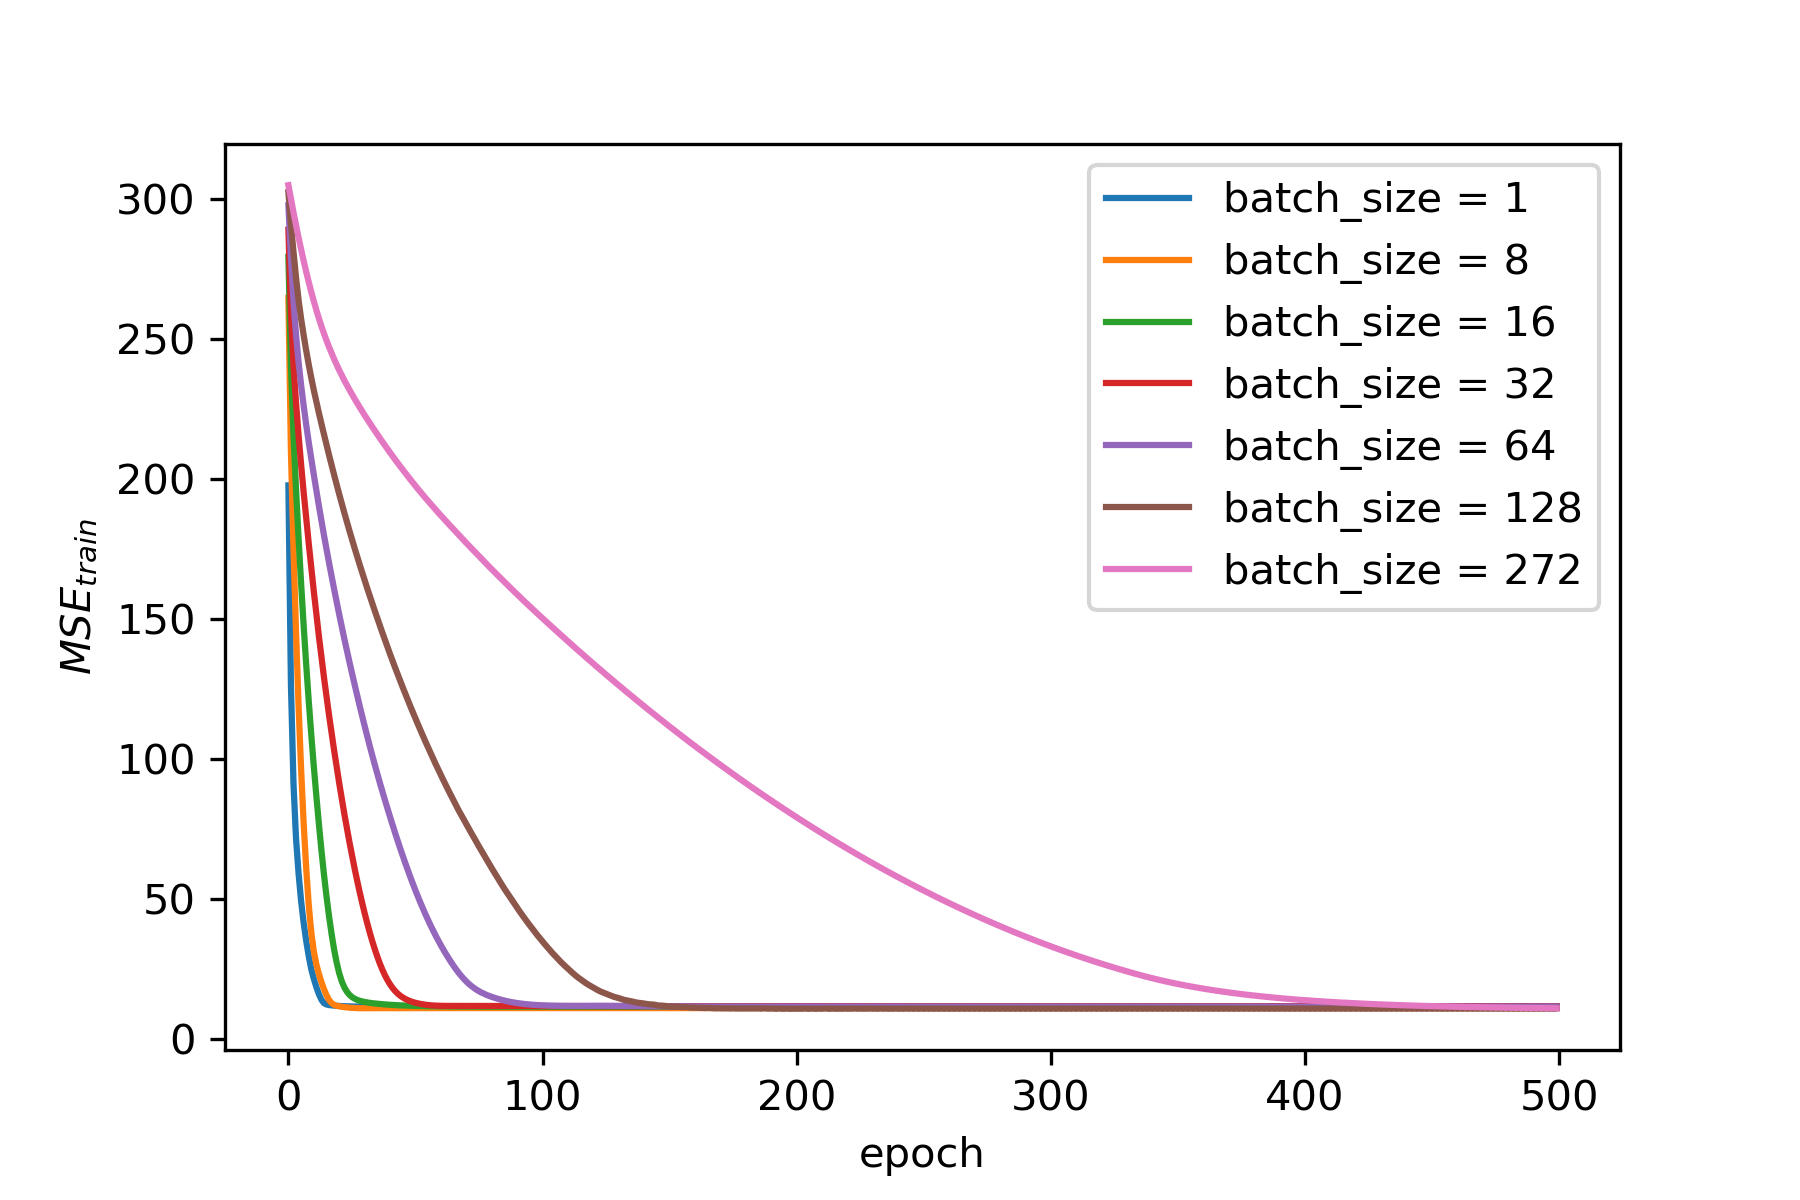
\includegraphics[width=\columnwidth]{batch_size_train}
		% Create a subtitle for the figure.
		\caption{The $MSE$ of training set under different batch size.}
		% Define the label of the figure. It's good to use 'fig:title', so you know that the label belongs to a figure.
		\label{fig:batch_size_train}
	\end{center}
\end{figure} 

\begin{figure}[!hbt]
	% Center the figure.
	\begin{center}
		% Include the eps file, scale it such that it's width equals the column width. You can also put width=8cm for example...
		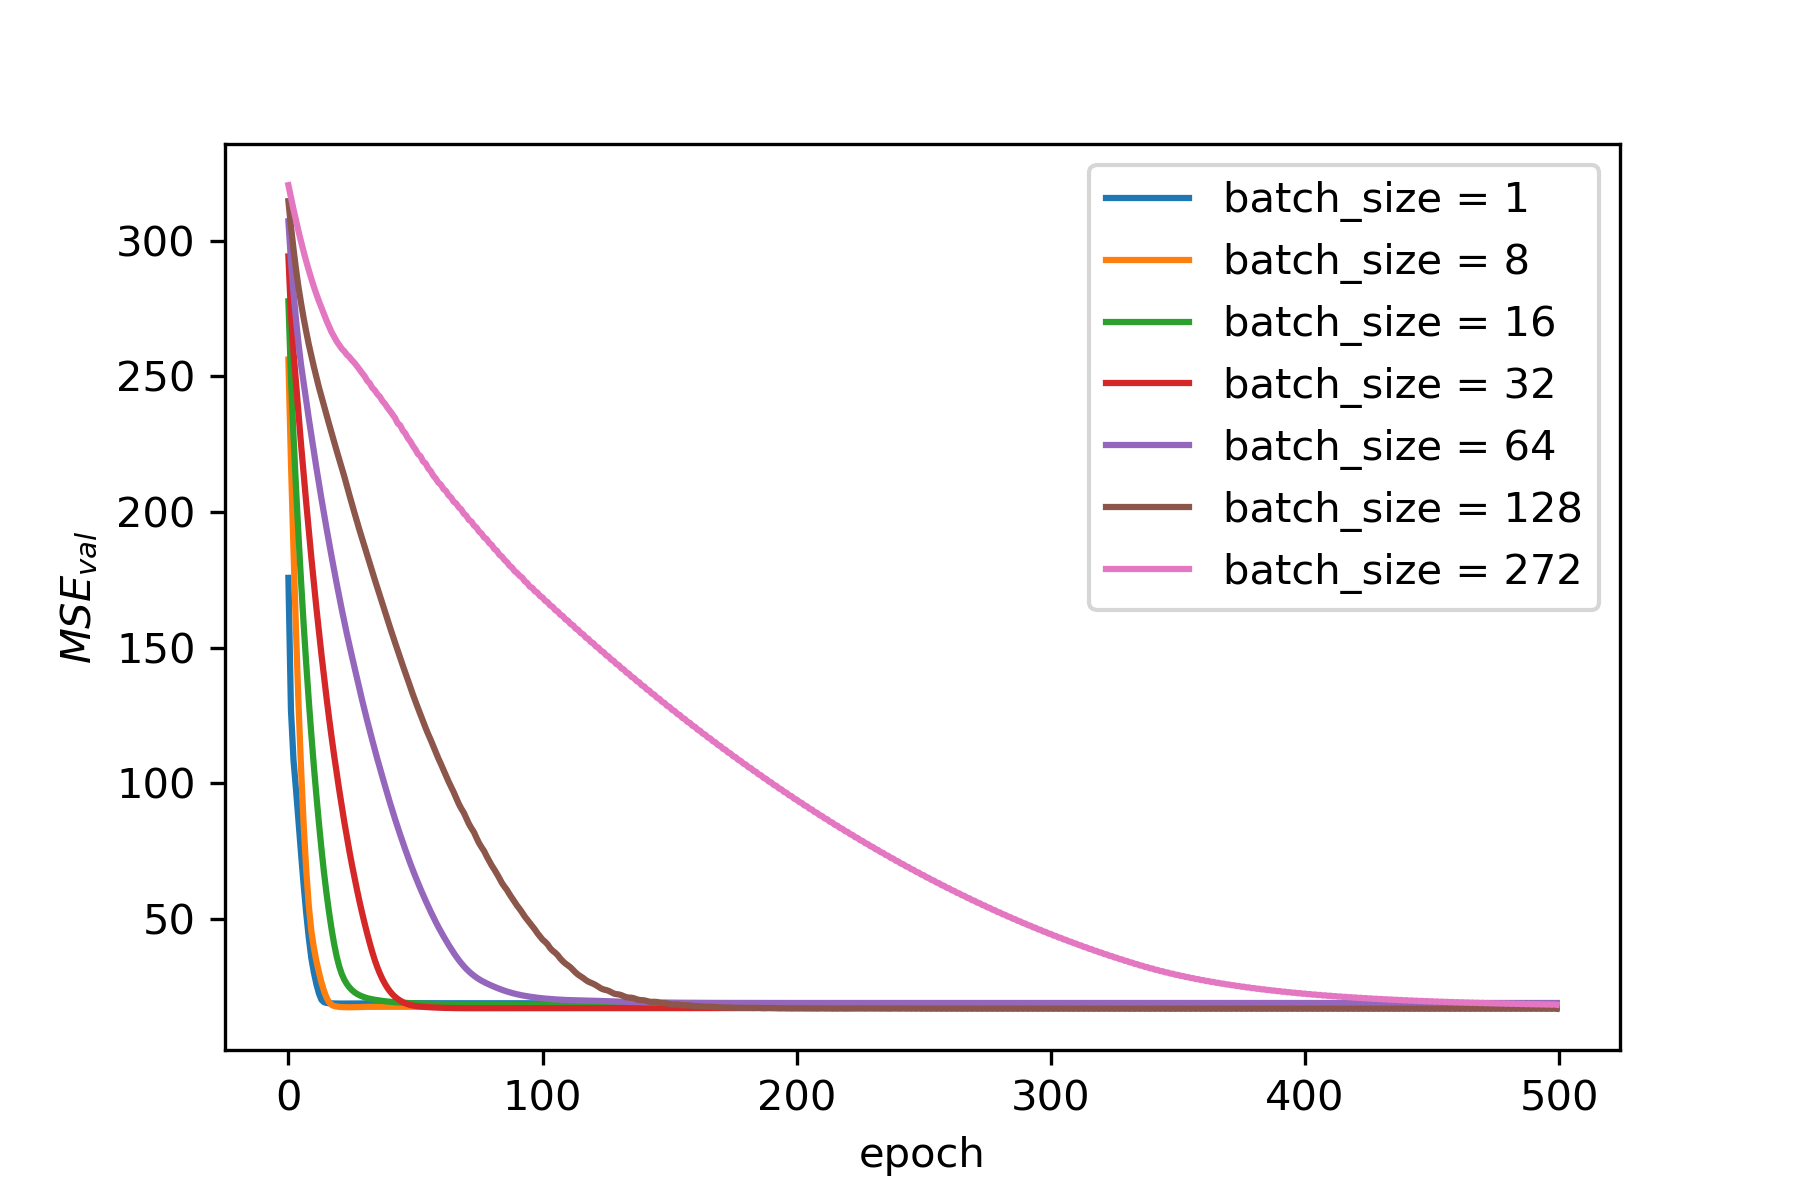
\includegraphics[width=\columnwidth]{batch_size_val}
		% Create a subtitle for the figure.
		\caption{The $MSE$ of validation set under different batch size.}
		% Define the label of the figure. It's good to use 'fig:title', so you know that the label belongs to a figure.
		\label{fig:batch_size_val}
	\end{center}
\end{figure} 

\begin{figure}[!hbt]
	% Center the figure.
	\begin{center}
		% Include the eps file, scale it such that it's width equals the column width. You can also put width=8cm for example...
		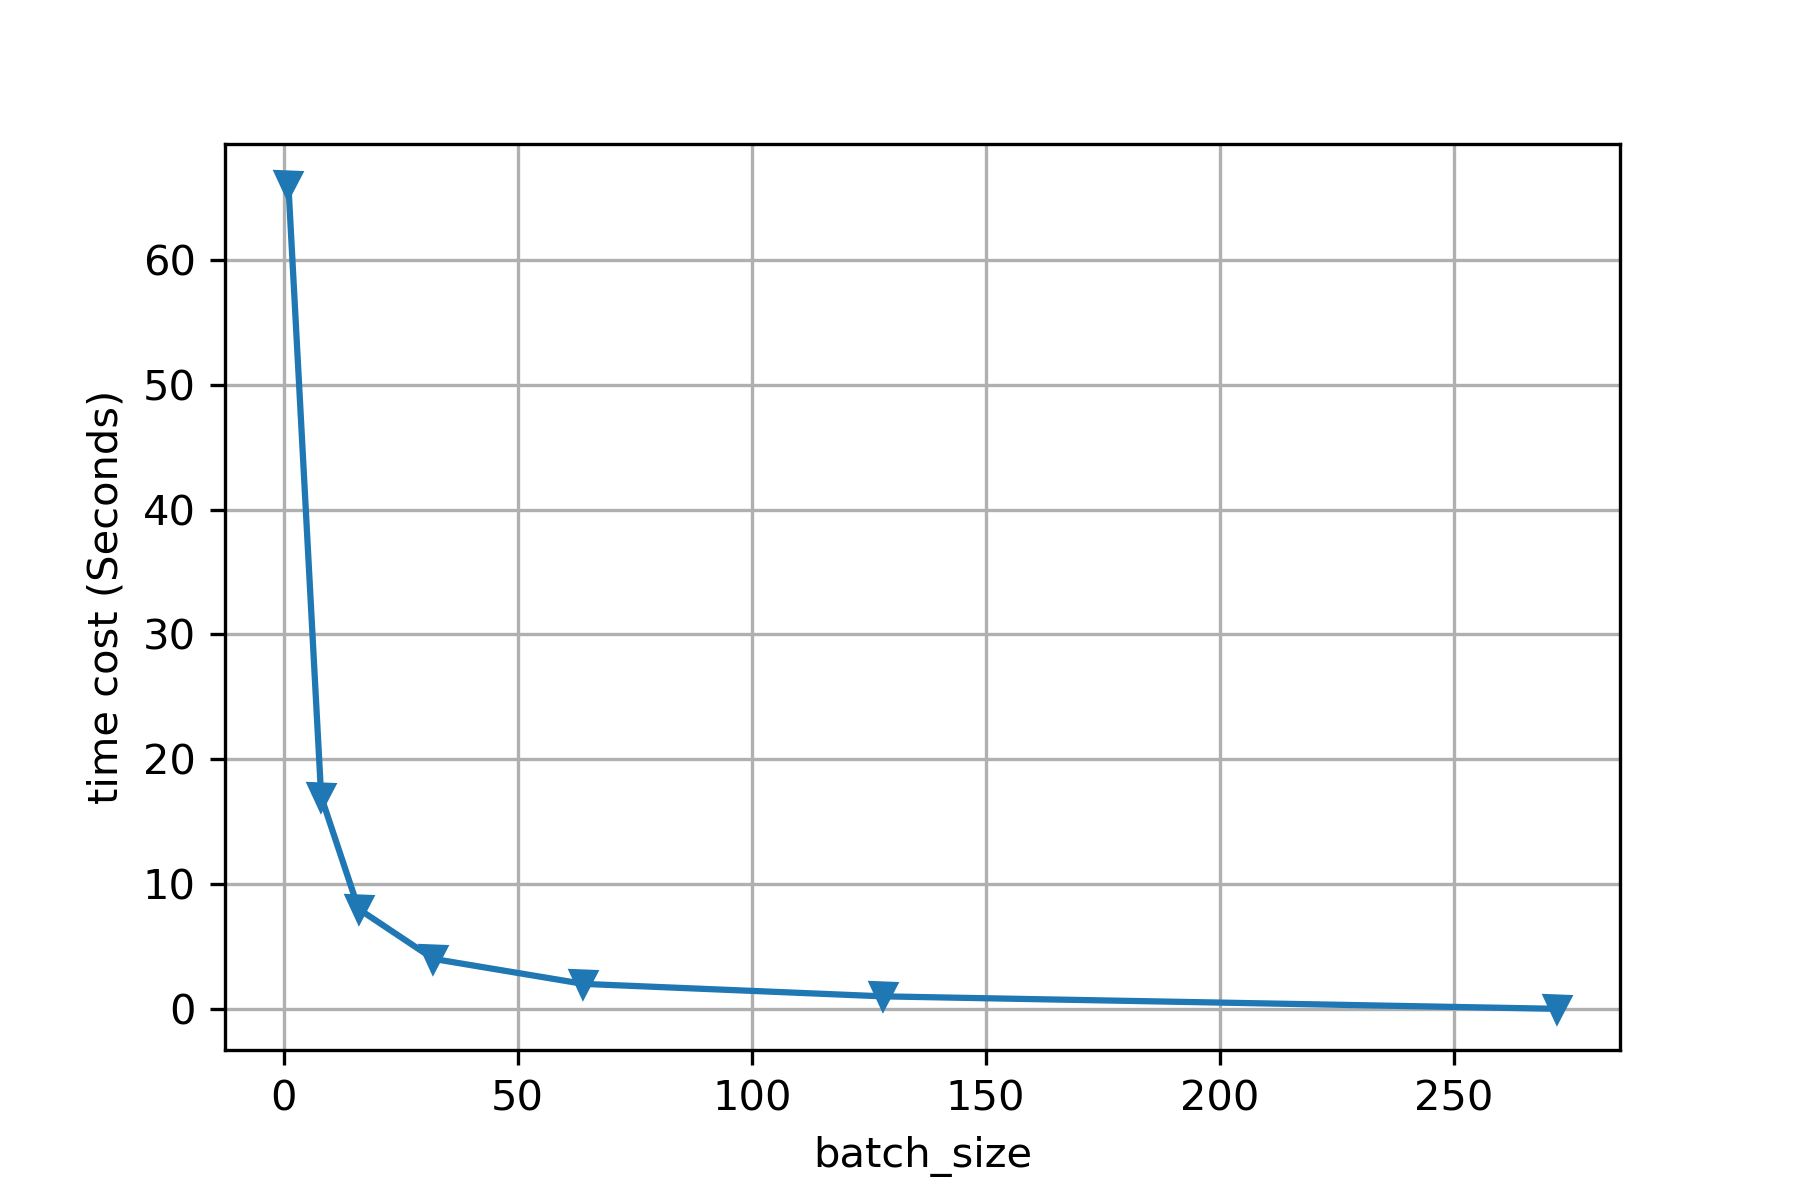
\includegraphics[width=\columnwidth]{time_cost}
		% Create a subtitle for the figure.
		\caption{The time cost of 100 epoches under different batch size.}
		% Define the label of the figure. It's good to use 'fig:title', so you know that the label belongs to a figure.
		\label{fig:time_cost}
	\end{center}
\end{figure} 

\subsection{Impact of learning rate}
In this section, we evaluate the impact of learning rate in MBGD, we set batch size to 64 and epochs to 200. We set learning rate in a range e.g. 1e-4, 1e-3, 1e-2, 1e-1, 1. \par
As presented in Fig~\ref{fig:lr_train} and Fig~\ref{fig:lr_val}, small learning rate tends to make the convergence smoothly, but needs more epoches to fully converge. However, big learning rate make the convergence very fast, but will not guarateee that the convergence will be near the optimal(or local optimal) and makes the $MSE$ shaking around after a specific epoch.  \par

\begin{figure}[!hbt]
	% Center the figure.
	\begin{center}
		% Include the eps file, scale it such that it's width equals the column width. You can also put width=8cm for example...
		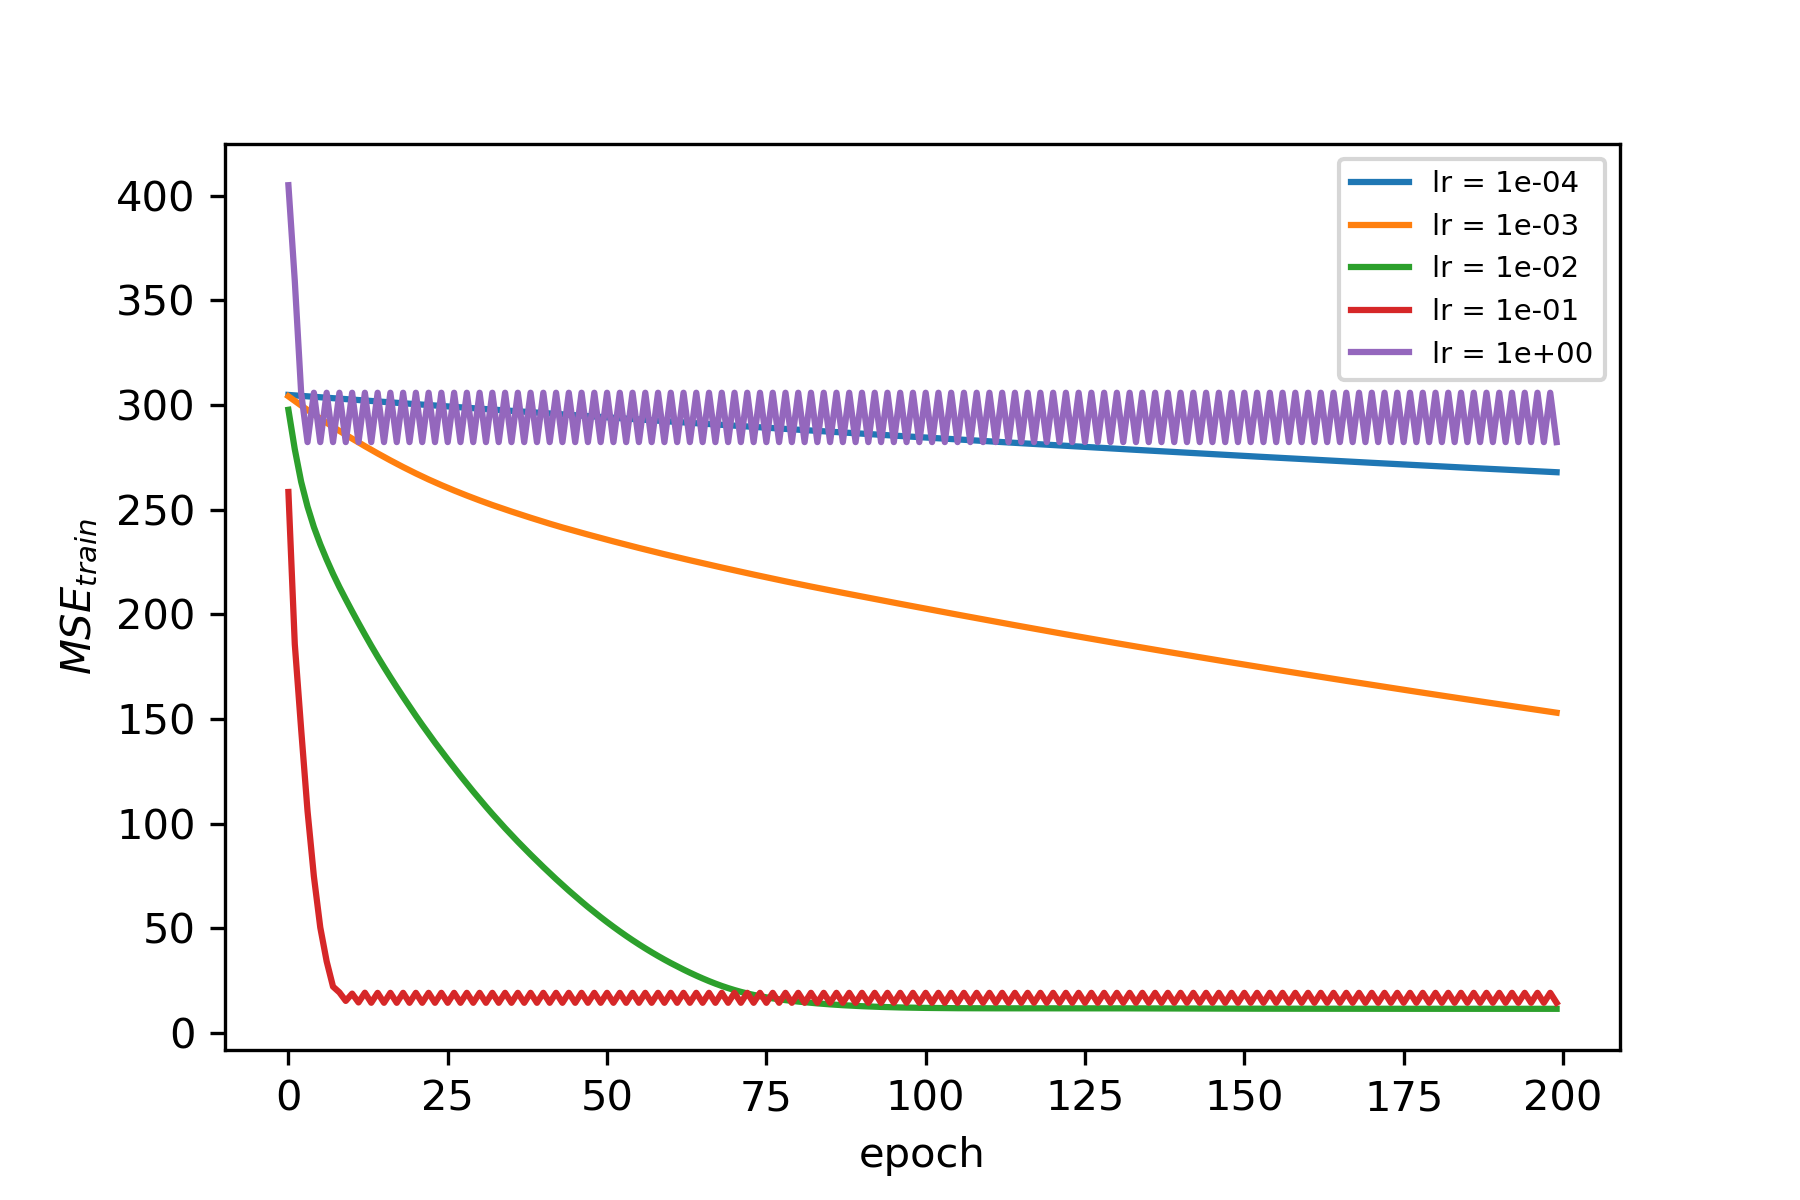
\includegraphics[width=\columnwidth]{lr_train}
		% Create a subtitle for the figure.
		\caption{The $MSE$ in training set under different learning rate.}
		% Define the label of the figure. It's good to use 'fig:title', so you know that the label belongs to a figure.
		\label{fig:lr_train}
	\end{center}
\end{figure} 

\begin{figure}[!hbt]
	% Center the figure.
	\begin{center}
		% Include the eps file, scale it such that it's width equals the column width. You can also put width=8cm for example...
		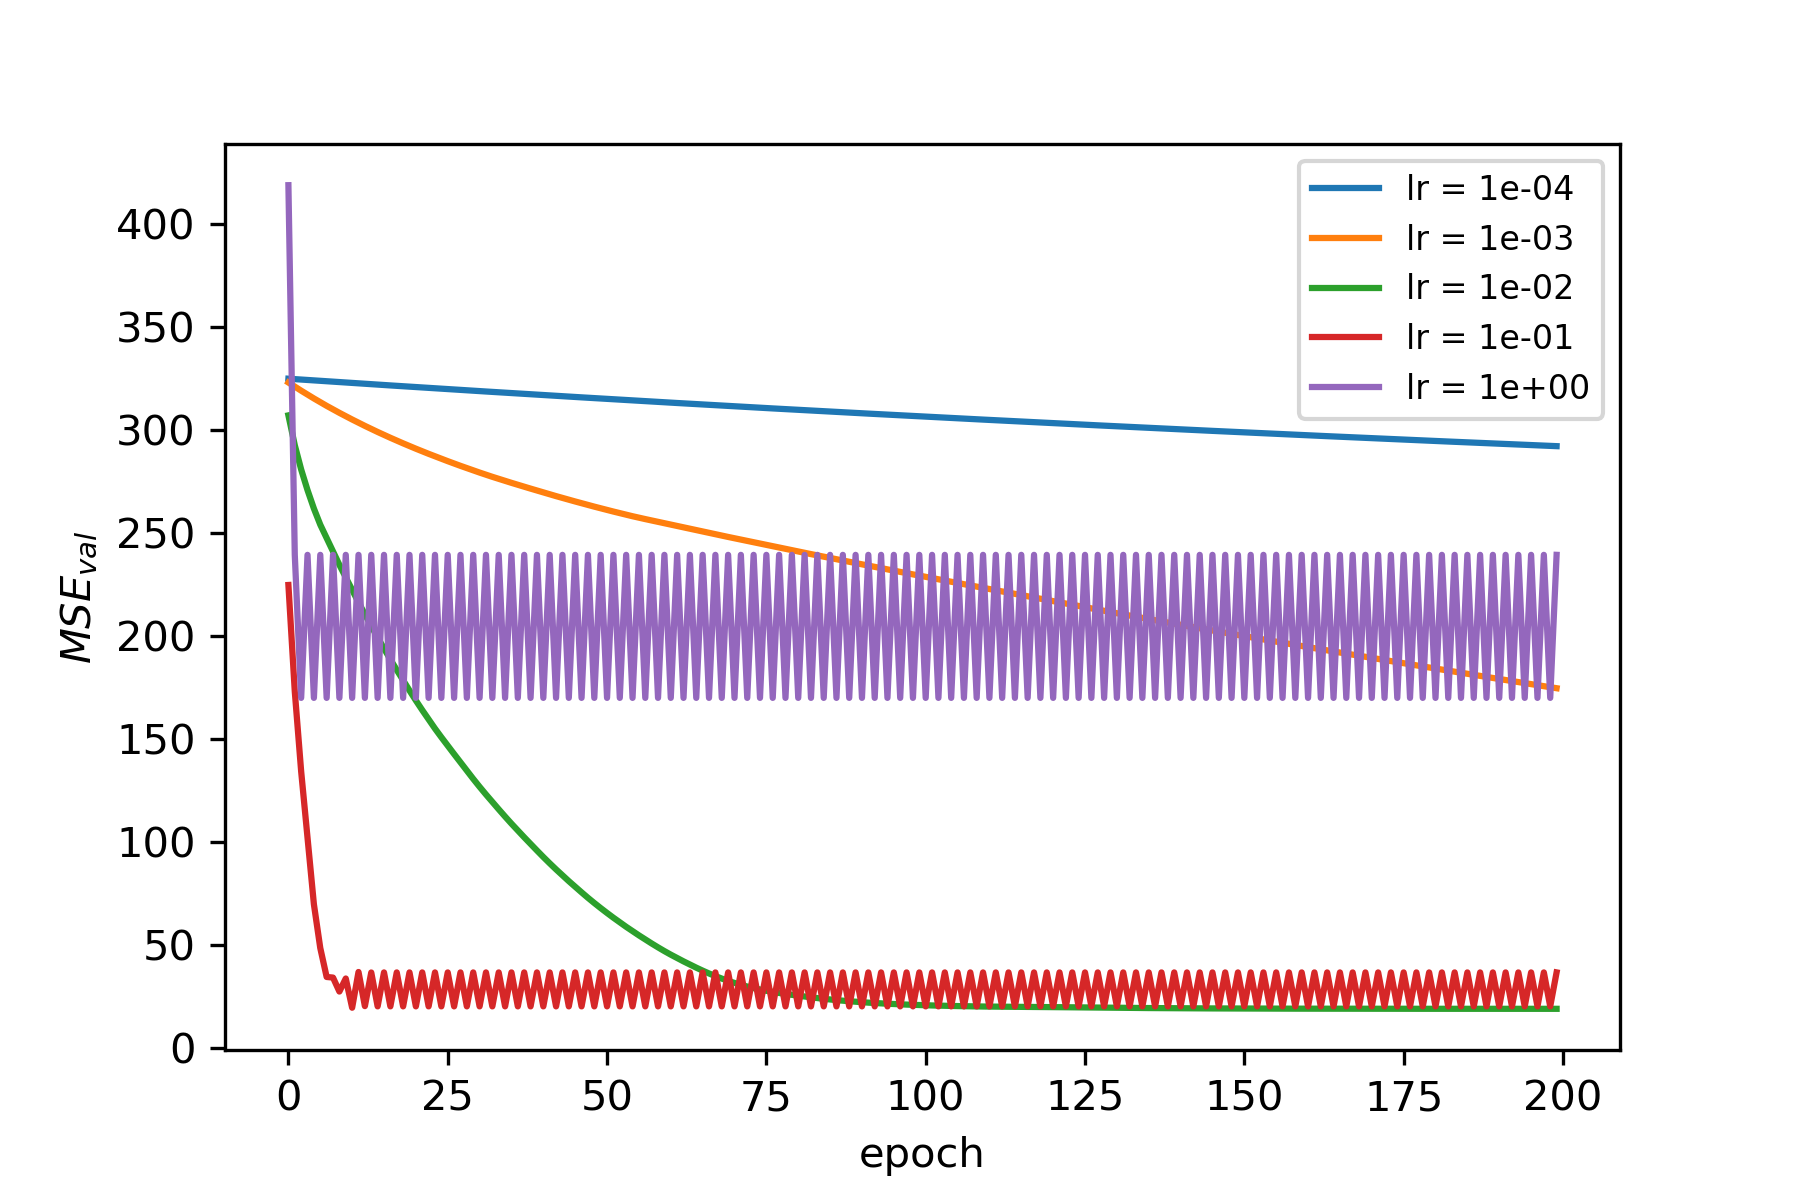
\includegraphics[width=\columnwidth]{lr_val}
		% Create a subtitle for the figure.
		\caption{The $MSE$ in validation set under different learning rate.}
		% Define the label of the figure. It's good to use 'fig:title', so you know that the label belongs to a figure.
		\label{fig:lr_val}
	\end{center}
\end{figure} 

\subsection{Weight magnitude between CSF and MBGD}
In this section, we explore the weight magnitude($L_2norm$) between CSF and MBGD optimized weight of linear regression. \par

Then, we experiments on comparing the weight magnitude of CFS and MBGD optimized LR. In MBGD, we set learning rate to 0.01 and batch size to 64. We can see that MBGD optimized LR's weight magnitude is stable after some epoches. But MBGD optimized weight's magnitude has a large margin(e.g. about 0.6) to CFS optimized weight. The reason is still unclear. \par

\begin{figure}[!hbt]
	% Center the figure.
	\begin{center}
		% Include the eps file, scale it such that it's width equals the column width. You can also put width=8cm for example...
		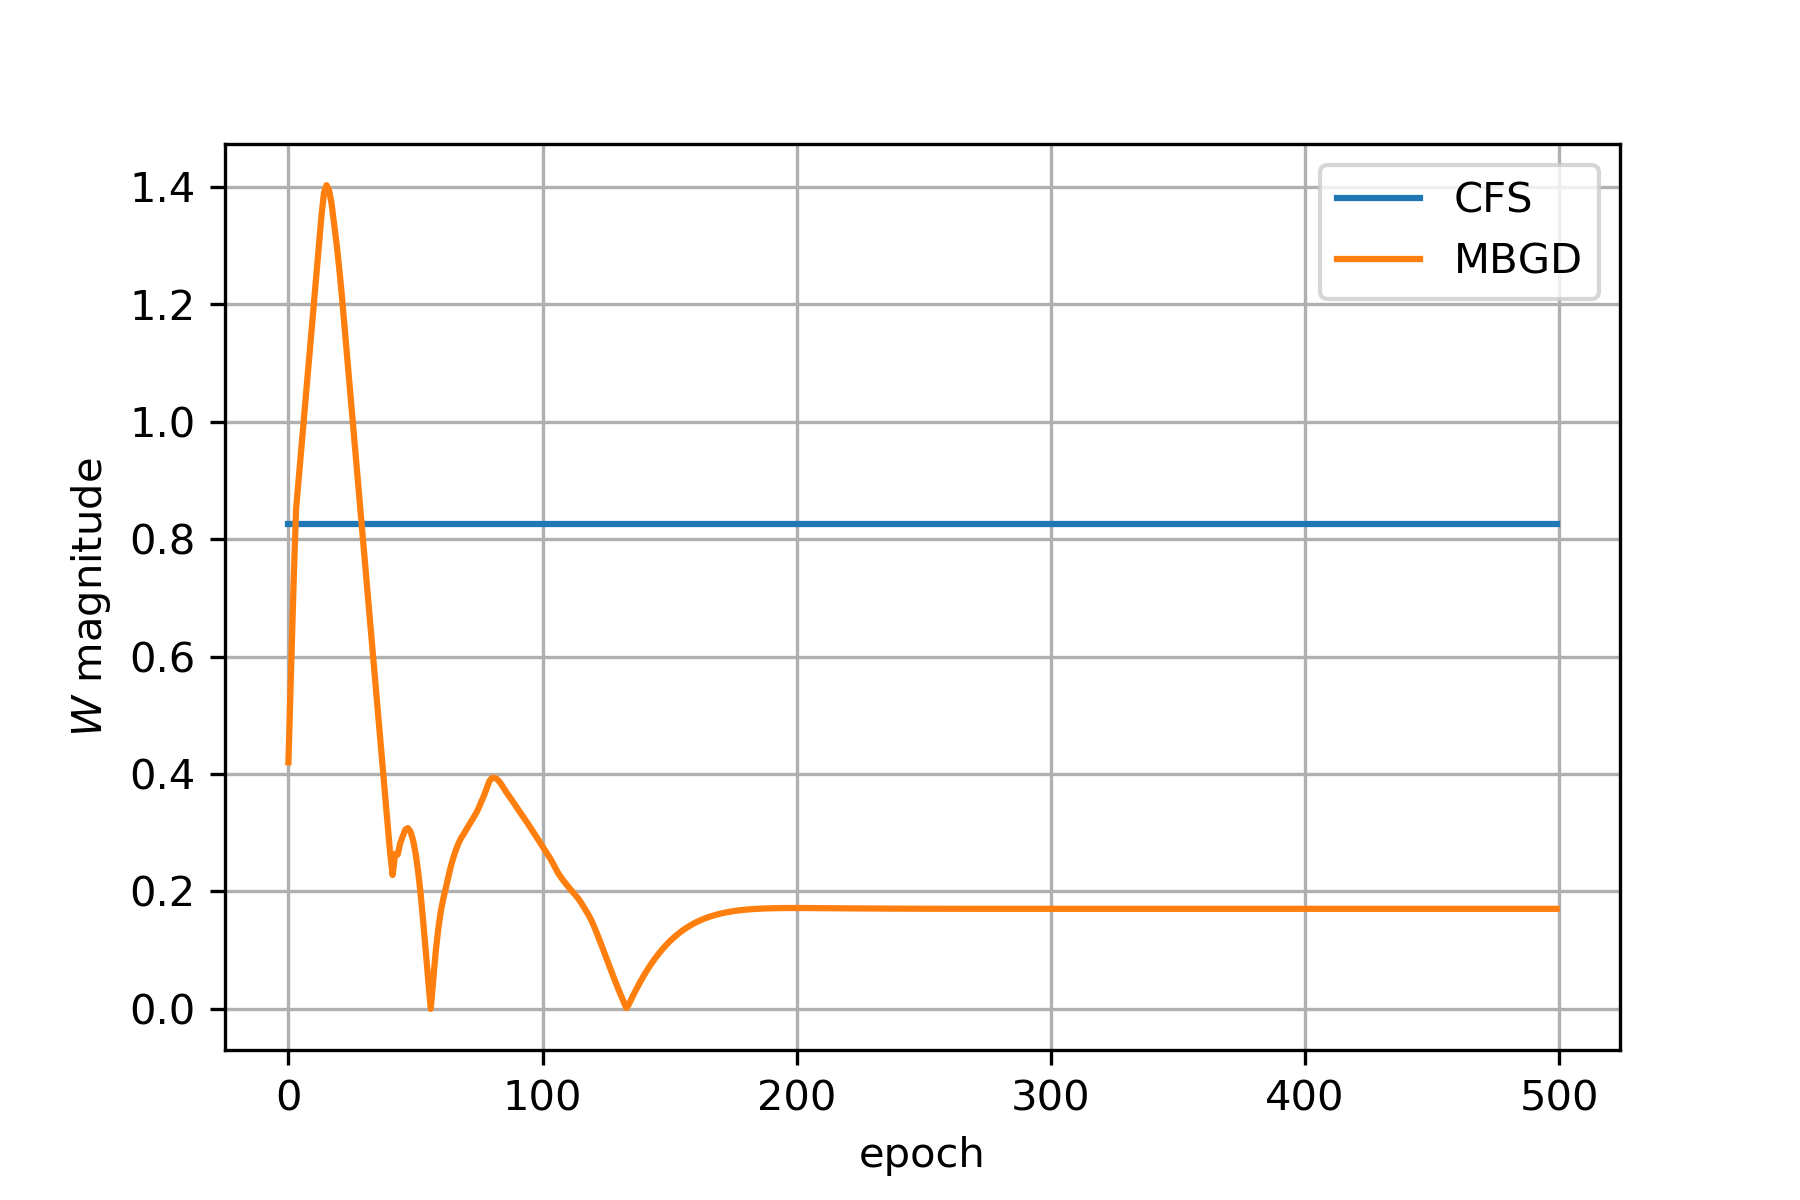
\includegraphics[width=\columnwidth]{mbgd_w}
		% Create a subtitle for the figure.
		\caption{The magnitude of $W_{mbgd}$ under different epoches..}
		% Define the label of the figure. It's good to use 'fig:title', so you know that the label belongs to a figure.
		\label{fig:mbgd_w}
	\end{center}
\end{figure} 

\subsection{Performance} 
In this section, we report the performance on CFS optimized LR, RR and MBGD optimized LR in training set, validation set and test set. The $\lambda$ is set to 1e-7 after validation. And batch size is set to 64 in MBGD, learing rate set to 0.01 and epoch set to 200 by validation. \par
From Table~\ref{tab:Performance}, we can see that alougth MBGD optimized LR's $MSE_{train}$ and $MSE_{val}$ are not the best, but its result in $MSE_{test}$ is outstanding. The reason remains unclear, maybe the same reason that the magnitude between CFS optimized LR and MBGD optimized LR has a large margin. \par
\begin{table}[!hbt]
	% Center the table
	\begin{center}
		% Title of the table
		\caption{Final Performance of CFS optimized LR, RR and MBGD optimized LR, best result are in bold.}
		\label{tab:Performance}
		% Table itself: here we have two columns which are centered and have lines to the left, right and in the middle: |c|c|
		\begin{tabular}{|c|c|c|c|}
			% To create a horizontal line, type \hline
			\hline
			% To end a column type &
			% For a linebreak type \\
			& LR & RR & MBGD \\
			\hline
			$MSE_{train}$   & \textbf{10.23} & \textbf{10.23} & 11.37   \\
			\hline
			$MSE_{val}$  & \textbf{17.08} & \textbf{17.08} & 19.04   \\
			\hline
			$MSE_{test}$  & 10.20 &  10.20 & \textbf{10.14}  \\
			\hline
		\end{tabular}
	\end{center}
\end{table}

\section{Conclusion}
In this report, we explore the CFS optimized LR, CFS optimized RR and MBGD optimized LR. We conduct the experiments on the CFS optimized LR and RR in terms of performance and weight magnitude. We also explore GD, SGD, MBGD in terms of convergence and time efficiency. Moreover, we tuning the hyper-parameter learning rate in MBGD. We also compare the weight magnitude between CFS optimized LR and MBGD optimized LR. Finally, we report the performance in CFS optimized LR, RR and MBGD LR. After a series of experiments, we now get more insight of LR, RR and GD and its variants SGD and MBGD. \par



% Your document ends here!


\end{document}